\chapter{Referencial Teórico}
\label{cap-referencial}

Nesse capítulo faremos um resumo dos principais conceitos envolvidos com o tema analisado.


%Aqui é fazer instrodução ao BI
%Falar de Plataforma de BI
%Falar das tecnologias envolvidas
%Posso colocar de anexo o Landscape do Matt Turck
%Dizer que existem diversas possibilidades de montar o lego
%Dizer que após o estudo chegaremos na proposta 
%E ai não é só comprar BI
%Tem que comprar BI, ETL e DW
%Separar Camada de Apresentacao, Camada de ETL e Camada de DW
%\section{Business Intelligence}
%Falar do Conceito de BI do Forrester


% \section{Visão Geral}
% \TODO{Fazer a partir do Turban}

% Um sistema de suporte à decisão é um conjunto de componentes inter-relacionados que coletam, processam, armazenam e distribuem informações destinadas a apoiar a tomada de decisões.

% O termo ``sistema de suporte à decisão'' tem sido utilizado cada vez menos na literatura e atualmente podemos dizer que esse conceito foi modernizado. Deste modo, sistemas desse tipo passaram a ser chamados de ``sistemas de inteligência de negócios'', onde popularizou-se o termo em inglês e sua sigla: \emph{Business Intelligence} (BI). Esse termo foi sugerido por Howard Dresner em 1989, como uma expressão abrangente para descrever ``conceitos e métodos para melhorar a tomada de decisões de negócios usando sistemas de suporte baseados em fatos'' \cite{dressner1986}.


\section{Plataformas de \emph{Business Intelligence}}
\label{sec-pĺataformasdebi}

\epigraph{``O começo é a parte mais difícil do trabalho.''}{\textit{Platão}}

Nada mais intuitivo do que começar pelo começo. Então vamos começar o desenvolvimento deste referencial teórico examinando o título deste estudo: 

\begin{env-destaque}{Titulo}
``Estudo Técnico sobre Plataformas de \emph{Business Intelligence}''. 
\end{env-destaque}

E assim podemos começar indagando:

\begin{quote}
\textbf{O que é uma Plataforma de \emph{Business Intelligence}?}
\end{quote}

Mas para responder essa pergunta precisamos investigar primeiro:

\begin{quote}
\textbf{O que é \emph{Business Intelligence}?}
\end{quote}

\subsection{\emph{Business Intelligence}}
\label{sub-bi}

Inteligência de Negócios (BI - \emph{Business Intelligence}) é um termo guarda-chuva que combina arquiteturas, ferramentas, bases de dados, ferramentas analíticas, aplicativos e metodologias. Trata-se de uma expressão de livre conteúdo, com significados diferentes de uma pessoa para outra. Parte da confusão provém da enxurrada de siglas e expressões associadas ao termo \cite{turban2019}. 

Portanto, atualmente existem diversas definições para BI dentre as quais destaca-se o conceito da companhia de pesquisas de mercado \emph{Forrester Research}:

\begin{definition}[\emph{Business Intelligence}]
\emph{Business Intelligence} é um conjunto de metodologias, processos, arquiteturas e tecnologias que transforma dados brutos em informações úteis e significativas usadas para possibilitar \emph{insights} e decisões estratégicas, táticas e operacionais mais eficazes \cite[tradução livre]{forrester:bi}.
\end{definition}
\index{Business Intelligence}

Agora, após termos definido BI, podemos nos aventurar e tentar entender o que que são Plataformas de BI.

\subsection{Plataformas de \emph{Business Intelligence}}
\label{sub-platbi}

Seguindo o raciocínio, chegou a vez de investigar o que são Plataformas de \emph{Business Intelligence} e, se possível, identificar empresas capazes de nos fornecer esse tipo de serviço.

Contudo, o próprio conceito de BI apresentado na seção anterior é tão amplo e tão genérico que o mercado oferece um vasto número de produtos tecnológicos relacionados com esse tema. Dessa feita, uma forma de organizar essa vastidão de tecnologias é agrupar e mapear as diversas soluções em grupos de categorias e subcategorias de soluções. Uma proposta de organizar essa vastidão de tecnologias relacionadas com dados é apresentada no panorama ``DATA \& AI LANDSCAPE 2019'' (ver Anexo \ref{anexo-landscape}) desenvolvido pelo executivo de \emph{venture capital} Matt Turck \cite{mattturck:principal}. 

Esse panorama apresenta a visão de um verdadeiro ecossistema de tecnologias relacionadas com dados e inteligência artificial dentre as quais encontramos a categoria de ``\emph{BI Platforms}'' que estamos interessados. A figura \ref{fig:landscape:bi} apresenta um recorte deste panorama. 

        \begin{figure}[htbp!]
            \centering
            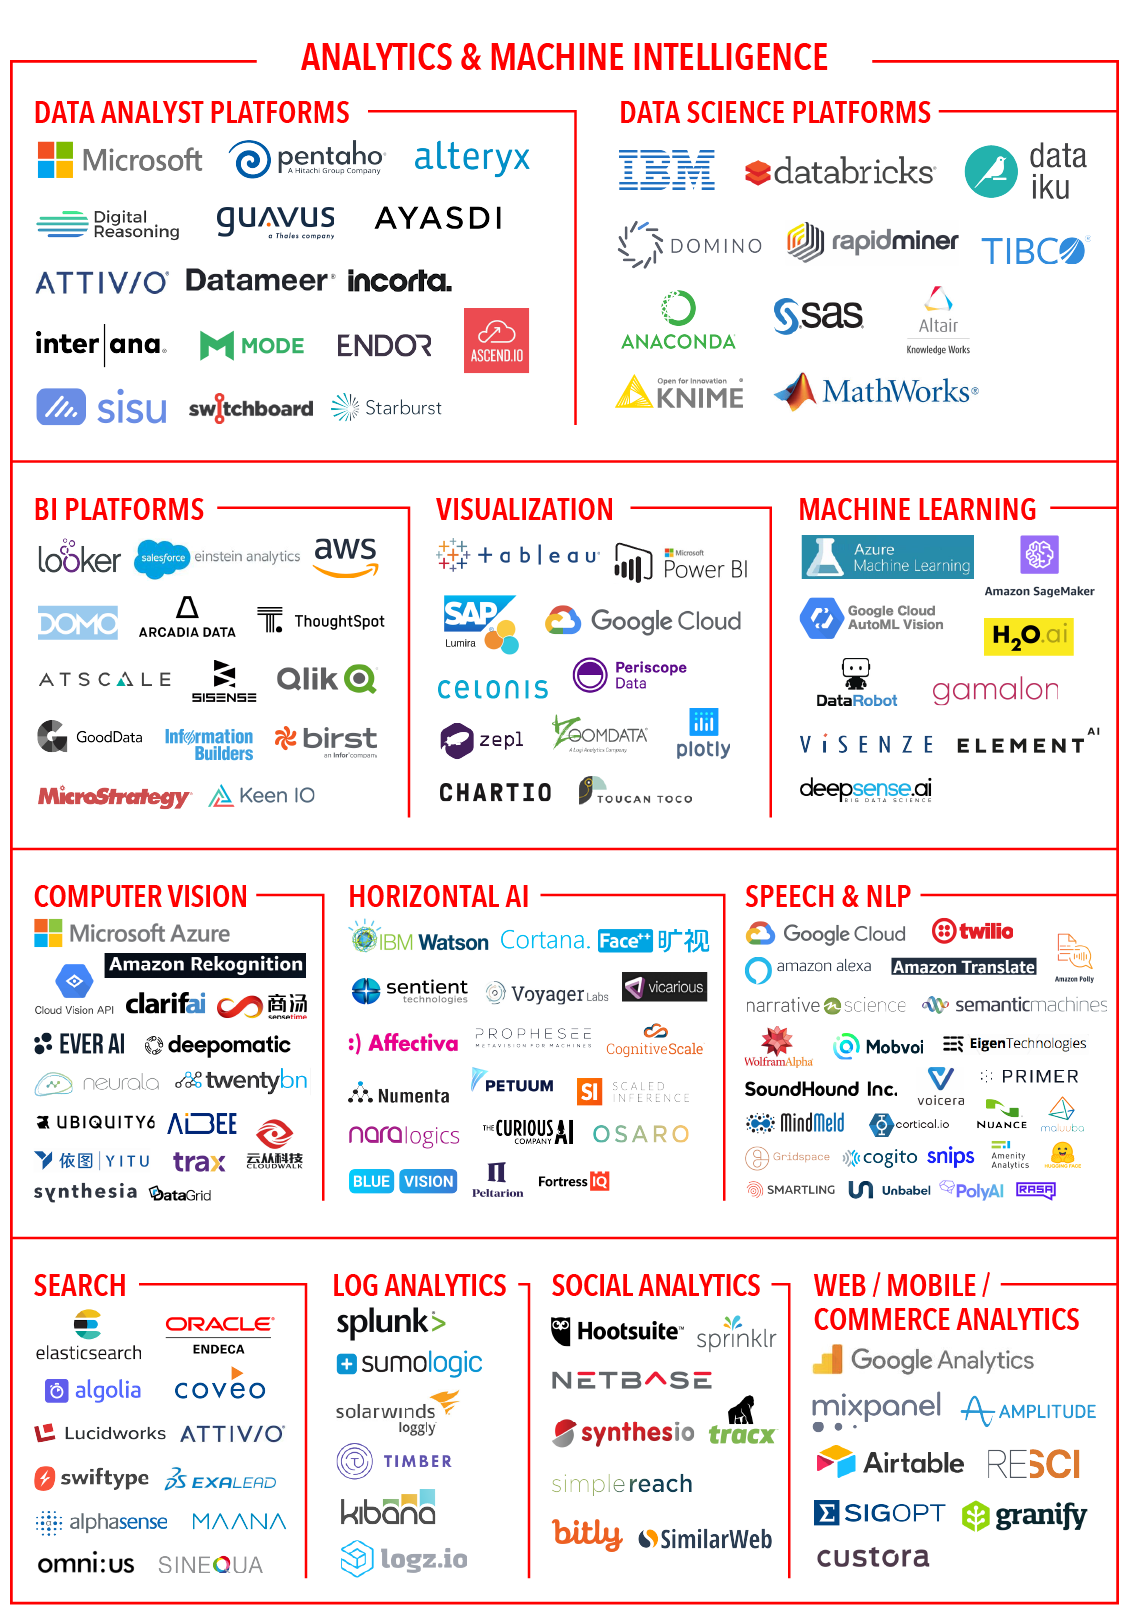
\includegraphics[width=0.8\textwidth]{fig/fig-panorama-biplatform.png}
            \caption{Recorte do Panorama ``DATA \& AI LANDSCAPE 2019'' de Matt Turck. Fonte: \cite{mattturck:principal}}
            \label{fig:landscape:bi}
        \end{figure}

Entretanto, mais uma vez, esse panorama que deveria nos ajudar acaba criando mais confusão pois descobrimos que a categoria de ``\emph{BI Platforms}'' é na verdade uma sub-categoria dentro de uma categoria maior denominada ``\emph{Analytics \& Machine Intelligence}''. Além disso, descobrimos que essa categoria de fornecedores aparece ao lado de uma série de categorias irmãs como, por exemplo: 
\emph{Data Analyst Platforms}, 
\emph{Data Science Platforms}, 
\emph{Visualization}, 
\emph{Machine Learning}, 
\emph{Computer Vision},
\emph{Horizontal AI},
\emph{Speech \& NLP},
\emph{Search},
\emph{Log Analytics},
\emph{Social Analytics},
\emph{Web / Mobile / Commerce Analytics}. Finalmente, o exame minucioso do panorama revela que  muitos fornecedores aparecem em mais de uma categoria.

Assim, a análise deste panorama levando em conta o conceito de BI definido na seção \ref{sub-bi} permite-nos fazer algumas observações:

\begin{enumerate}
    \item Como era de se esperar, existem diversas metodologias para transformar dados em informações. Portanto, existem também uma infinidade de produtos especializados em cada etapa desse processo. Por exemplo, alguns produtos se especializaram em recursos de Visualização de Dados enquanto outros em Visão Computacional e assim por diante. E é por isso que o panorama apresenta diversas outras categorias.
    
    \item Uma Plataforma de BI é um conjunto de ferramentas especializadas, geralmente de um mesmo fornecedor, que se integram para permitir que dados sejam analisados. Porém, algumas plataformas oferecem mais recursos que outras. Por exemplo, a plataforma de determinado fornecedor pode concentrar-se nos aspectos de visualização dos dados enquanto a plataforma de outro fornecedor concentra-se no suporte às operações de acesso, extração, carregamento, tratamento e preparação dos dados. E muitas vezes, podem existir plataformas que cobrem mais de uma funcionalidade.  
\end{enumerate}

Neste mundo de possibilidades, precisamos determinar o que buscamos. Nesse sentido, o Grupo \emph{Gartner} em um dos seus diversos artigos técnicos nos inspirou a criar a seguinte definição para ``Plataformas de \emph{Business Intelligence}'', que retrata o que esperamos de uma solução dessas:

\begin{definition}[Plataformas de \emph{Business Intelligence}]
Plataformas de \emph{Business Intelligence} modernas são sistemas que oferecem suporte ao desenvolvimento de conteúdo analítico através de uma arquitetura autocontida que permite que usuários não técnicos executem fluxos de trabalho analíticos de forma autônoma, desde o acesso e preparação dos dados até a análise interativa e compartilhamento colaborativo de \emph{insights} \cite[tradução livre,adaptado]{gartner:biplatforms}.
\end{definition}
\index{Plataformas de Business Intelligence}

Certamente, esse conceito de Plataformas de \emph{Business Intelligence} apresentado acima servirá de bússola para nos ajudar a navegar nesse mar de tecnologias de dados. 

\section{Análise de Dados e o BI}

\epigraph{``\emph{Data is the new oil. It’s valuable, but if unrefined it cannot really be used. It has to be changed into gas, plastic, chemicals, etc to create a valuable entity that drives profitable activity; so must data be broken down, analyzed for it to have value.}''}{\textit{Clive Humby}\footnote{Os dados são o novo óleo. É valioso, mas se não for refinado, não pode realmente ser usado. Tem que ser transformado em gás, plástico, produtos químicos, etc. para criar uma entidade valiosa que impulsione a atividade lucrativa; assim, os dados devem ser decompostos, analisados para que tenham valor. \cite[tradução livre]{epigrafes:dataisthenewoil}}}


    Nessa seção pretendemos resumir o conceito de análise de dados, o que isso tem a ver com BI e porque entender esses conceitos é importante neste estudo. 

\subsection{Os três níveis de Análise de Dados}
\label{sub-niveis}

    A expressão \emph{análise de dados} pode ser compreendida como:
    
    \begin{definition}[Análise de Dados]
    O processo de desenvolvimento de decisões ou recomendações práticas para ações baseadas em vislumbres gerados por dados históricos. \cite[23]{turban2019} 
    \end{definition}
    \index{Análise de dados}
    
    Dessa forma, muitos proponentes e acadêmicos utilizam hoje a expressão \emph{análise de dados} no lugar de BI. Isto têm um porquê que será explicado adiante.
    
    Diferentes organizações propõe suas próprias interpretações e motivações para a análise de dados, entretanto a literatura técnica tem concordado no sentido de propor três níveis de análise de dados: análise descritiva, análise preditiva e análise prescritiva. 
    
        \begin{figure}[h]
            \centering
            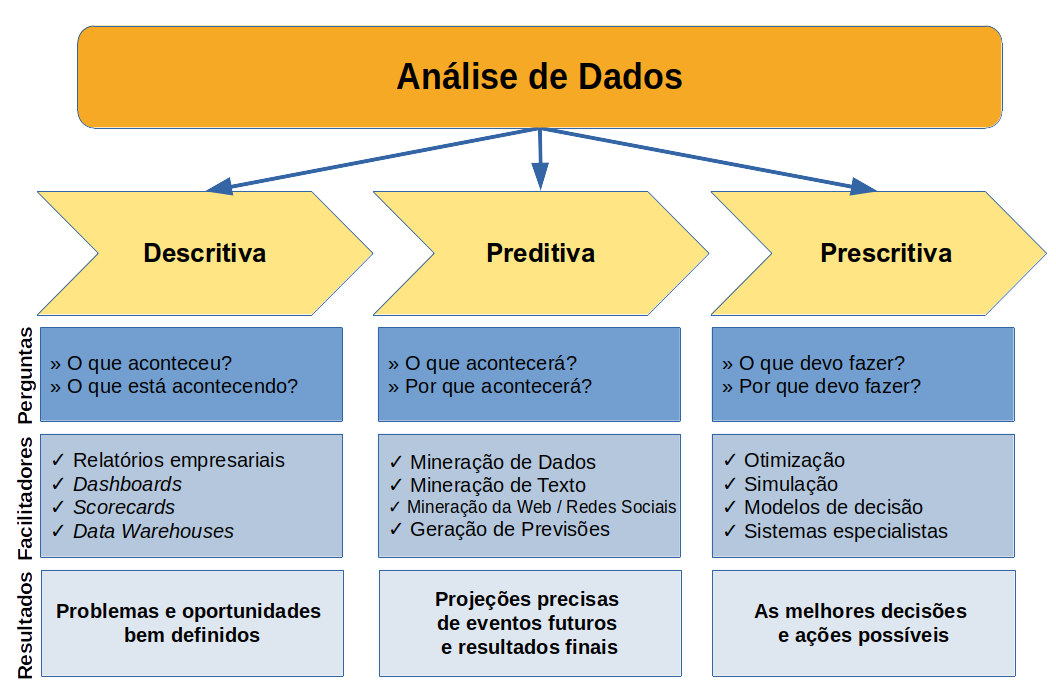
\includegraphics[width=\textwidth]{fig/fig-analise-niveis.png}
            \caption{Os três tipos de análises de dados. Fonte: \cite[adaptado]{turban2019}.}
            \label{fig:analise:niveis}
        \end{figure}
    
    
    A figura \ref{fig:analise:niveis} apresenta uma visão gráfica desses três níveis e sugere que esses níveis representam etapas de certa forma independentes e que um tipo de aplicação de análise de dados leva a outro. Além disso, a figura sugere que há também uma certa sobreposição entre esses três tipos de análise de dados. Seja como for, a natureza interconectada dos diferentes tipos de análise de dados fica evidente. Além disso, a figura apresenta quais perguntas cada nível de análise de dados pretende responder, os facilitadores e os resultados esperados da aplicação bem sucedida de cada etapa \cite[24]{turban2019}. 

\subsection{E o BI?}
\label{sub-eobi}

    Conforme \emph{Ramesh Sharda et al.} afirmam \cite[153]{turban2019}, o termo inteligência de negócios (BI), que já vêm circulando a mais de 20 anos como um termo para descrever decisões gerenciais tomadas com base em evidências e fatos, perdeu seu lugar como ``expressão da moda'' para este novo termo ``\emph{análise de dados}''. Assim, hoje em dia, \textbf{BI é usado para descrever os estágios iniciais da análise de dados, isto é, a análise de dados descritiva}.
    
    \begin{figure}[h]
        \centering
        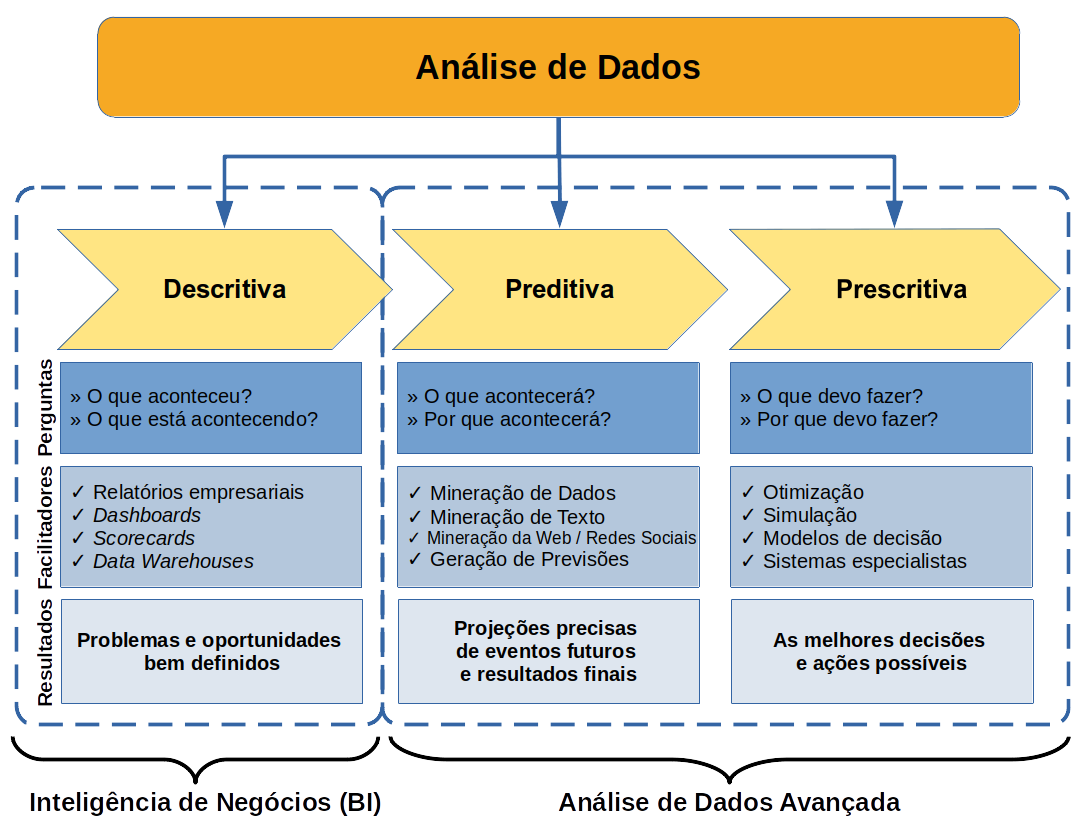
\includegraphics[width=\textwidth]{fig/fig-analise-bi.png}
        \caption{Inteligência de Negócios (BI) e Análise de Dados Avançada. Fonte: \cite[adaptado]{turban2019}.}
        \label{fig:analise:bi}
    \end{figure}
    
    Dessa forma, a figura \ref{fig:analise:bi} apresenta uma nova versão da figura \ref{fig:analise:niveis}. Verifique que o BI refere-se à análise de dados descritiva (primeiro nível de análise de dados) cuja maturidade leva a análise de negócios avançada - uma combinação de análise de negócios preditiva e prescritiva.

\subsection{\emph{Analytics}}

    Neste cenário, aparece outro termo, que com certeza também têm se popularizado. Estamos falando do termo: \emph{Advanced Analytics} ou simplesmente  \emph{Analytics}. O \emph{analytics} é o termo em inglês para se referenciar à análise de dados avançada (preditiva e prescritiva) identificada na figura \ref{fig:analise:bi}.

\subsection{BI e BA}
\index{Business Analytics}

    E já que estamos falando de termos da moda, se por um lado existe BI então porque não BA? Se BI é a sigla de \emph{Business Intelligence}, então o leitor adivinhou corretamente que BA é a sigla para \emph{Business Analytics}. 

\subsection{Plataformas de ABI}
\index{Plataformas de ABI}

    Novamente, se existem Plataformas de BI então porque não falar de Plataformas de BA? Porque geralmente as plataformas de BA também oferecem recursos de BI. Veja que o amadurecimento em BI é condição para realizar BA. Deste modo, se uma plataforma quer oferecer serviços de BA, ela precisa, no mínimo, oferecer o nível de análise de dados anterior, ou seja, o BI. 
    
    Assim chegamos no termo utilizado pelo Grupo \emph{Gartner} para definir o mercado de análise de dados. Essa instituição usa o termo ``\emph{Analytics and Business Intelligence Platforms}'' (\emph{ABI Platforms}) para se referir às principais plataformas qualificadas para oferecer recursos de análise de dados descritiva, preditiva e prescritiva a seus clientes.
    
    Finalmente, neste estudo, em vez de traduzir esse termo para ``Plataformas de Inteligência de Negócios e Análise de Dados Avançadas'' escolhemos, por simplicidade, utilizar o termo original ``Plataforma de BI'' ou até mesmo ``Plataforma de ABI'' para nos referir a essas soluções de análise de dados.
    

\section{Por que \emph{Plataforma}?}
\label{sec-porqueplat}

    Já concentramos nossa atenção nos termos \emph{Business Intelligence}, \emph{Analytics} e até já oferecemos um conceito para Plataforma de BI conforme seção \ref{sub-platbi}. Contudo, é fundamental discutir o porquê do termo  \emph{plataforma}.

    Então, para ressaltar a importância dessa discussão, repetimos a pergunta dessa seção:
    
    \begin{env-destaque}{Pergunta}
    \begin{quote}
        Por que \emph{Plataforma}?
    \end{quote}
    \end{env-destaque}

    Vamos retomar a definição apresentada de  Plataformas de \emph{Business Intelligence} e dessa vez vamos destacar uma determinada palavra-chave:
    
    \begin{quote}
        ``Plataformas de \emph{Business Intelligence} modernas são \large \textbf{sistemas} \normalsize que oferecem suporte ao desenvolvimento de conteúdo analítico através de uma arquitetura (...)'' 
    \end{quote}
    
     Portanto, é muito importante entender que uma solução de análise de dados é constituída de um \textbf{sistema} de ferramentas. Veja a definição de ``sistema'': 
    
    \begin{quote} 
     ``Um sistema é um conjunto de elementos interdependentes de modo a formar um todo organizado'' \cite{wikipedia:sistema}.
    \end{quote}
    
    Muitas vezes emprestamos o termo ``ecossistema'' da biologia para ressaltar o fato de que uma plataforma de BI é constituída de um conjunto de outros sistemas de software e hardware. E assim, cada fornecedor oferece seu próprio conjunto de sistemas.
    
    \begin{quote} 
        Então, por que \emph{plataforma}?
    \end{quote}
    
    \begin{env-destaque}{Resposta}
    \begin{quote}
        Porque geralmente um ambiente de análise de dados depende de diversas ferramentas e cada fornecedor oferece seu próprio conjunto particular delas: uma \emph{plataforma} de ferramentas de BI.
    \end{quote}
    \end{env-destaque}
    
    \subsection*{Não confundir a parte com o todo}
     
     Nesse cenário, dentre as diferentes ferramentas de um ecossistema de análise de dados, a que mais ``aparece'' e portanto 
     torna-se o ``carro-chefe'' de um determinado fornecedor é a ferramenta de \textbf{visualização de dados}.  E assim, muitas vezes a parte é confundida com o todo pois um ambiente completo de análise de dados necessita de muitos outros recursos além da construção de \emph{dashboards} e criação de gráficos.
     
     Distinguir o todo da parte é fundamental, e para isso, vamos apresentar a ``Jornada dos Dados'' e assim entender que tipos de ferramentas são utilizadas em cada etapa dessa jornada.
     
\section{Jornada dos Dados}    
\label{sub-jornadadosdados}

    \begin{figure}[htbp!]
        \centering
        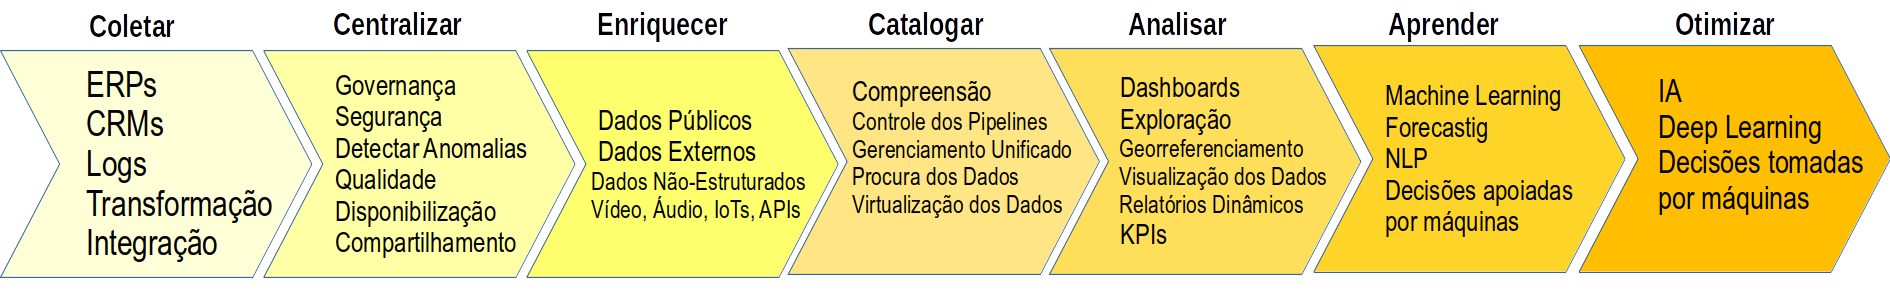
\includegraphics[width=\textwidth]{fig/fig-jornada.png}
        \caption{Jornada dos Dados. Fonte: \cite[adaptado]{a10:jornada}.}
        \label{fig:jornadadados}
    \end{figure}

    A figura \ref{fig:jornadadados} apresenta a jornada de dados. Cada etapa dessa jornada será explicada e sempre que possível, ferramentas de mercado identificadas por \emph{Matt Turck} \cite{mattturck:sheet} serão exibidas. Além disso, utilizaremos o cenário de implantação do ambiente de análise de dados da \CODEPLAN \xspace (CODEPLAN) para exemplificar. 

    \subsection{Geração dos Dados}

    Embora não esteja na figura \ref{fig:jornadadados}, os dados são gerados pelos sistemas de informação que administram as transações de negócio sobre o qual vão se aplicar as análises e a inteligência de negócio. A título de exemplo, em um sistema que vai avaliar dados sobre o SUS, os dados são gerados, em sua maioria, pelos próprios sistemas de informação onde estão ocorrendo as transações do SUS, entre as quais, consultas médicas, compras de materiais etc.

    \subsection{Coletar, Transformar, Integrar}\label{acessos-dados}
    
    O insumo fundamental para a análise de dados e inteligência de negócios são exatamente os dados brutos. Esses dados encontram-se sob gestão daqueles que operam os sistemas de informação dos ambientes transacionais. Para isso, faz-se necessário que o gestor do ambiente analítico acesse esses dados, para então usá-los como insumo. Esse acesso pode ser feito de diversas maneiras:

\begin{itemize}
    \item \textbf{Uma única vez}: nesse caso, obtêm-se o dado relativo a um único momento, relativo ao estado da base de origem daquele momento da captura. Esse dado pode ser transmitido por qualquer meio possível, e será armazenado no repositório analítico da (\emph{data warehouse} ou \emph{datalake}). Todas as análises que serão feitas, só levarão em consideração o estado dos dados no momento da captura.
    \item \textbf{Periodicamente}: nesse caso, obtêm-se o dado relativo a um momento, e passa-se a atualizá-lo com determinada periodicidade. O dado é armazenado no repositório analítico, podendo ser armazenada somente a versão mais atual ou então um acúmulo de versões capturadas. Existem diversas abordagens de atualização e armazenamento aplicáveis, cada qual mais adequada para um determinado contexto. Essa captura periódica pode ser feita manual ou automaticamente, porém recomenda-se o uso de captura automatizada, de modo a se garantir a padronização da forma de captura, além de se economizar em recursos humanos de atividades repetitivas e automatizáveis. Vale lembrar que o acesso aos dados é utilizado a cada captura, devendo ser mantido pelo gestor do sistema transacional enquanto durarem as capturas. Trata-se da estratégia mais utilizada no meio de BI.
    \item \textbf{Em tempo real}: nesse caso, o sistema de origem dos dados comunica-se com o sistema de captura, de modo que esses sincronizam esforços para que os dados sejam transportados para a base analítica à medida em que há atualização neles. Essa estratégia apresenta importante ganho por trazer análises em tempo real, porém o seu custo pode ser considerado por vezes muito elevado, o que faz dela pouco utilizada.
\end{itemize}

Após realizada a coleta dos dados, a literatura aponta para o passo de transformação deles. A transformação é necessária, pois não existe a premissa de que os dados coletados estarão todos eles adequados a um mesmo padrão, que seja adequado à análise. De certo, em geral, a forma como os dados são armazenados nas bases transacionais e nas analíticas é diferente, pois o foco de cada uma é bastante diverso.

A transformação é feita por \emph{software} próprio que consiste em realizar operações sobre os dados coletados. Alguns exemplos dessas operações são citados abaixo:

\begin{itemize}
    \item \textbf{Padronização de termos sinônimos}: termos sinônimos devem ser padronizados, de modo a facilitar o trabalho de inteligência posterior. Exemplo disso são bases que utilizem as Unidades Federativas. Essas unidades podem ser colocadas na forma de sigla ou por extenso. Independentemente da forma escolhida, é importante de se padronizar uma forma, para aumentar a eficácia dos motores de inteligência. É muito comum que os dados coletados não sejam homogêneos nesse sentido; por exemplo, numa coleta de dados das Secretarias de Estado, pode-se observar que a Secretaria de Saúde adote o formato de siglas, enquanto a Secretaria de Segurança Pública adote o formato extenso. Apesar de não haver erros nas bases, no momento em que ambas serão levadas para um mesmo repositório, é importante se estabelecer um padrão.
    \item \textbf{Resumo}: em alguns casos, pode-se concluir que não se necessita de toda a granularidade dos dados transacionais para as bases analíticas. A título de exemplo, suponhamos os dados da Secretaria de Saúde sobre consultas médicas, onde a base transacional possua dados de cada consulta realizada. Pode ser uma decisão do projeto que a base analítica vai guardar apenas os dados diários de consultas por unidade de saúde, ao invés dos dados individualizados das consultas.
    \item \textbf{Anonimização}: com o advento da Lei Geral de Proteção de Dados -- LGPD, existem alguns cuidados que devem ser utilizados sempre que um dado pessoal for tratado. Para isso, no caso do tratamento a ser dado pela base analítica não estar compreendido nas hipóteses juridicamente possíveis sobre aquele dado, ele deve ser anonimizado, de modo que deixa de ser considerado dado pessoal.
    \item \textbf{Estruturação de dados não estruturados}: os dados podem estar de forma não estruturada na fonte. É o caso de imagens e vídeos. Entretanto, pode-se extrair metadados deles, de modo que a saída seja formada por metadados. Por exemplo, no caso de a origem conter uma imagem com 5 megapixels, pode-se extrair o metadado relativo ao tamanho da imagem, decidindo-se armazenar a mera informação de que trata-se de uma imagem com 5 megapixels, ao invés de se armazenar a imagem propriamente dita. Ainda, pode-se utilizar um software para reconhecer elementos na imagem e se armazenar uma descrição desses elementos, ao invés da imagem em si.
\end{itemize}

A transformação deve ser feita de modo automatizado, prioritariamente, sendo configurada dentro de software específico, que esteja preparado para ter como entrada o dado conforme coletado, e como saída o dado, conforme deve ser integrado.

\begin{env-sistemas}{Exemplos de Ferramentas de Coleta e Transformação de Dados}
     \begin{multicols}{2}
        \begin{itemize}
            \item \emph{Alteryx}
            \item \emph{AWS Athena}
            \item \emph{AWS Glue}
            \item \emph{Azure Data Factory}
            \item \emph{Fishtown Analytics}
            \item \emph{Kalido}
            \item \emph{Lattice Data}
            \item \emph{Paxata}
            \item \emph{Pentaho}
            \item \emph{Revelytix}
            \item \emph{StreamSets}
            \item \emph{StrikeIron}
            \item \emph{Talend}
            \item \emph{Tamr}
            \item \emph{Trifacta}
        \end{itemize}
    \end{multicols}
\end{env-sistemas}

Após devidamente transformado, esse dado será integrado à solução de armazenamento analítico. Esse passo consiste em armazenar esse dado em meio não volátil, dentro do conjunto de soluções de armazenamento analítico.

\begin{env-sistemas}{Exemplos de Ferramentas de Integração de Dados}
     \begin{multicols}{2}
        \begin{itemize}
            \item \emph{Alooma (Google)}
            \item \emph{Attunity (Qlik)}
            \item \emph{Bedrock Data (Formstack)}
            \item \emph{Enigma}
            \item \emph{Fivetran}
            \item \emph{Import.io}
            \item \emph{MuleSoft (Salesforce)}
            \item \emph{Podium Data (Qlik)}
            \item \emph{Talend}
            \item \emph{Tealium}
            \item \emph{Xplenty}
            \item \emph{Zaloni}
        \end{itemize}
    \end{multicols}
\end{env-sistemas}

Aqui, deve-se tomar algumas considerações. No caso de dados estruturados, esses são armazenados em uma estrutura chamada \emph{data warehouse}, à medida em que os dados não estruturados são armazenados em uma estrutura chamada \emph{datalake}. Ambientes mais simples consistem apenas de \emph{data warehouse}. Nesse sentido, recomenda-se a implementação do \emph{data warehouse} num primeiro momento, deixando o \emph{datalake} para implementação futura, tendo em vista a maior complexidade e investimento a ser feito.

\begin{env-sistemas}{Exemplos de Sistemas de \em{Data Warehouses}}
     \begin{multicols}{2}
        \begin{itemize}
            \item \emph{Amazon Redshift}
            \item \emph{Azure Synapse}
            \item \emph{Google BigQuery}
            \item \emph{Google Mesa}
            \item \emph{InfoWorks}
            \item \emph{Infoworks.io}
            \item \emph{Microsoft SQL Data Warehouse}
            \item \emph{Oracle Exadata Cloud}
            \item \emph{Pivotal Greenplum}
            \item \emph{Snowflake}
            \item \emph{SpaceCurve}
            \item \emph{IBM Data Warehouse Systems}
        \end{itemize}
    \end{multicols}
\end{env-sistemas}

O \emph{data warehouse} pode ser organizado de diversas maneiras. Uma delas consiste na criação de \emph{data marts} (repositórios específicos) que sejam feitos um para cada categoria (como tema de fiscalização, por exemplo). Outra forma é a criação de uma base única. 

    \begin{env-caso}{Caso CODEPLAN}
        Nessa etapa, a CODEPLAN organizou em planilhas, após 36 reuniões com os parceiros do governo, os responsáveis e o conjunto de informações estratégicas e de interesse da empresa. Foi criado dessa forma um catálogo de informações sobre esse conjunto de informações contendo tanto informações internas quanto externas da empresa.
    \end{env-caso}

    \subsection{Centralizar} \label{sec:centralizar}
    
    Uma vez que já existe um repositório analítico de dados, onde os dados se encontram prontos e acessíveis para a análise, deve-se pensar em uma centralização desses dados. Isso ocorre, pois muito provavelmente esses dados se encontram em uma diversidade de ferramentas de armazenamento, tendo-se em vista que existem dados estruturados (em \emph{data warehouse}) e dados não estruturados (em \emph{datalake}), e que ainda pode haver uma variedade de instâncias e ferramentas dentro de cada um. Assim, pode haver a existência de uma ferramenta que centralize a gestão sobre esses dados, que ocorra num único lugar. 

    \begin{env-sistemas}{Exemplos de Ferramentas de Governança de Dados}
         \begin{multicols}{2}
            \begin{itemize}
                \item \emph{Alation}
                \item \emph{Colibra}
                \item \emph{Dremio}
                \item \emph{Immuta}
                \item \emph{Informatica}
                \item \emph{Okera}
                \item \emph{Sailpoint}
                \item \emph{Waterline Data}
            \end{itemize}
        \end{multicols}
    \end{env-sistemas}
    
    Outro aspecto importante é a segurança dos dados. Diversas são as opções de sistemas especializados em soluções de segurança. 

    \begin{env-sistemas}{Exemplos de Ferramentas de Segurança de Dados}
         \begin{multicols}{2}
            \begin{itemize}
                \item \emph{Blue Hexagon}
                \item \emph{CloudFlare}
                \item \emph{CyberX}
                \item \emph{Dataguise}
                \item \emph{Datavisor}
                \item \emph{Sqrrl (Amazon)}
                \item \emph{ThreatMetrix (Lexis Nexis)}
                \item \emph{Vade Secure}
                \item \emph{Accumulo (Open Source)}
                \item \emph{Knox (Open Source)}
                \item \emph{Ranger (Open Source)}
                \item \emph{Sentry (Open Source)}
            \end{itemize}
        \end{multicols}
    \end{env-sistemas}

    % http://dfkoz.com/ai-data-landscape/

    A centralização não é considerada um componente essencial em um ambiente ainda embrionário e pequeno, porém torna-se cada vez mais necessária à medida em que o ambiente cresce e torna-se complexo.

    \begin{env-caso}{Caso CODEPLAN}
        Como grande parte das informações são públicas, é concentrada a publicação\footnote{Nota-se que a CODEPLAN realizou uma centralização de publicação de dados, porém não informou sobre centralização da gestão, rastreamento e auditoria da camada de persistência analítica de dados.} dos dados no portal codeplan.df.gov.br e nas ferramentas do \#infoDF. Esse último, além de criar um repositório de dados nos SGBDs (PostgreSQL e SQLServer, ambos sob gestão da Subsecretaria de Tecnologia da Informação e Comunicação da Secretaria da Economia - SUTIC), disponibiliza os dados através de API's.
    \end{env-caso}

    
    \subsection{Enriquecer} \label{sec:enriquecer}
    
    
Com os dados centralizados, muitas ferramentas também possuem funcionalidades relacionadas ao enriquecimento desses dados. Trata-se da função de adicionar metadados ou fazer complementações manualmente ou proveniente de outras bases de dados, que estão fora do escopo daquelas usadas na origem dos dados. Exemplo disso se dá quando se recebe da \emph{wikipedia} detalhamento sobre dados existentes nas bases analíticas.

\begin{env-caso}{Caso CODEPLAN}
Os cruzamentos entre as bases foram feitos e disponibilizadas com o ElasticSearch, Python e clientes de banco de dados (Squirel e DBeaver).
\end{env-caso}
    
    \subsection{Catalogar} \label{sec:catalogar}
    
    Em havendo dados tratados, visíveis em uma única interface e devidamente enriquecidos, esses dados podem ser servidos de forma intuitiva para a montagem de análises e visualizações. Assim, algumas ferramentas criam a funcionalidade de catálogo, que traz o benefício de simplificar a criação de análises e visualizações por usuários leigos, de forma mais amigável, num ambiente \emph{self service}. Apesar de não ser uma funcionalidade essencial para um ambiente de BI, recomenda-se fortemente a sua adoção, de modo a aumentar a produtividade dos profissionais que criarão os painéis de visualização, trazendo ganho no longo prazo.


\begin{env-caso}{Caso CODEPLAN}
O catálogo foi criado no WordPress com o intuito de ser um cadastro rápido e simples. Isso foi fundamental para organizar o cadastro dos dados e seus produtores. A ideia é uma busca rápida livre, onde o usuário encontra rapidamente a organização que produz aquela informação pesquisada.
\end{env-caso}
    
    \subsection{Analisar} \label{sec:analisar}
    
    Um dos principais objetivos postulados quando do estabelecimento de um projeto de implantação de BI é a pretensão de se criar um painel de visualização que traga informações valiosas para a tomada de decisão. Além desse, a criação de alertas também figura dentre os mais cobiçados, em que deseja-se que a ferramenta proporcione avisos sobre determinadas situações que demandam uma ação.

    \subsubsection*{Ferramentas de Visualização}
    
    Por esse motivo, talvez as primeiras ferramentas que venham à mente quando se pensa no universo de BI e Análise de Dados sejam as ferramentas de visualização, que tem criado painéis cada vez mais intuitivos e interativos.

    \begin{env-sistemas}{Exemplos de Ferramentas de Visualização}
         \begin{multicols}{2}
            \begin{itemize}
                \item \emph{Actuate}
                \item \emph{Captain Dash}
                \item \emph{Celonis}
                \item \emph{Chartio}
                \item \emph{DataHero}
                \item \emph{Looker}
                \item \emph{Microsoft Power BI}
                \item \emph{Plotly}
                \item \emph{Tableau}
                \item \emph{Bokeh (Open Source)}
                \item \emph{Matplotlib (Open Source)}
                \item \emph{Seaborn (Open Source)}
                \item \emph{Superset (Open Source)}
                \item \emph{TensorBoard (Open Source)}
            \end{itemize}
        \end{multicols}
    \end{env-sistemas}

    Aqui vale a ressalva de que, em havendo uma ferramenta intuitiva de catálogo, pode-se até atribuir a montagem de painéis ao usuário final leigo, com pouco treinamento, à medida em que na ausência de um catálogo, passa a se requerer mais conhecimento específico da pessoa responsável pela montagem dos painéis.

    Em havendo uma ferramenta corporativa de visualização, os painéis são montados por um perfil de usuário, que deixa-os disponíveis em um repositório, sendo facilmente visualizáveis por quem tiver a permissão. As ferramentas mais modernas padronizaram essa visualização em formato web, sendo que os painéis podem inclusive ser colocados dentro de portais web, como elementos dinâmicos.

    \subsubsection*{Ferramentas de Alertas}

    Ademais dos painéis, há também as ferramentas que cuidam da geração de alertas\footnote{Não encontramos exemplos isolados de ferramentas de alertas porque geralmente esse recurso faz parte das ferramentas de visualização.}. Essas mantém a verificação sobre o atendimento de condições pré-estabelecidas, efetivando ações determinadas em caso de satisfação da condição, tal como o disparo de e-mails, o acendimento de semáforos em painéis dinâmicos, dentre outras possíveis. Essas ferramentas são de grande utilidade quando se deseja monitorar a ocorrência de fenômenos que implicam ação imediata pelo observador, tal como a fuga de um prisioneiro de um complexo penitenciário, que implica o informe às autoridades que estão na rua sobre a fuga e os dados do fugitivo. 

    \subsubsection*{Plataformas de BI}
    
    Nesse contexto cabe finalmente retomar as Plataformas de BI que foram introduzidas na seção \ref{sub-platbi}. Uma Plataforma de BI é geralmente um sistema de ferramentas dentre as quais destaca-se a ferramenta de visualização que pode contar com recursos adicionais inerentes às demais etapas da jornada de dados. As diversas ferramentas de visualização\footnote{As ferramentas de visualização de dados de destaque serão apresentadas e avaliadas no Capítulo \ref{cap-fornecedores}.} podem funcionar sozinhas oferecendo recursos básicos de transformação, integração de dados e análise como podem também operar em sistemas mais complexos onde são utilizadas em conjunto com diversas outras ferramentas descritas nesse capítulo. Por isso é importante entender essa jornada de dados para que seja possível construir o ambiente mais adequado às necessidades de análise de dados da instituição.

    \begin{env-caso}{Caso CODEPLAN}
        São utilizadas algumas ferramentas de BI, públicas e construídas, para realizar cruzamentos e montar dados mais robustos. Power BI, Tableau, AmCharts, Kibana e ElasticSearch são fundamentais para publicar e cruzar diversas informações de parceiros.
    \end{env-caso}
    
    \subsection{Aprender}\label{sec:aprender}
    
    Nessa etapa, a partir do amadurecimento das etapas anteriores, torna-se possível aplicar técnicas de análise de dados preditiva e prescritiva para aprender com os dados. Neste contexto é possível utilizar algoritmos de \emph{Machine Learning} e 
    técnicas de \emph{Data Mining} para apoiar a tomada de decisões.

    \subsection{Otimizar}\label{sec:otimizar}

    Nessa etapa, a instituição confia nos dados e utiliza técnicas avançadas de inteligência artificial para tomar decisões.  

    \begin{env-sistemas}{Exemplos de Sistemas de \emph{Machine Learning}, \emph{Deep Learning} e AI}
         \begin{multicols}{2}
            \begin{itemize}
                \item \emph{AlchemyAPI}
                \item \emph{Amazon Sagemaker}
                \item \emph{Azure ML Studio}
                \item \emph{Bonsai (Microsoft)}
                \item \emph{Cloud AutoML}
                \item \emph{DataRobot}
                \item \emph{Prediction.io}
                \item \emph{OpenAI (Open Source)}
                \item \emph{OpenML (Open Source)}
                \item \emph{PyML (Open Source)}
                \item \emph{PyTorch (Open Source)}
                \item \emph{Scikit-learn (Open Source)}
            \end{itemize}
        \end{multicols}
    \end{env-sistemas}

    \begin{env-exemplo}{Caso CODEPLAN}
        Alguns estudos e trabalhos, com parceiros externos como a Controladoria-Geral do Distrito Federal (CGDF), envolvem análises de sentimentos e processamento de linguagem natural (NLP).
    \end{env-exemplo}
    
    \index{CGDF}
    \index{NLP}